\documentclass{article}
\usepackage[a4paper, total={6in, 8in}]{geometry}
\usepackage{graphicx, tikz}
\usetikzlibrary{automata, positioning, matrix}
\usepackage{parskip, multicol, fancyhdr, float}
\usepackage{biblatex, hyperref}
\usepackage{amsmath, amssymb}
\addbibresource{sources.bib}
\usepackage{algpseudocode}
\fancyfoot[R]{\thepage}

\begin{document}
\section{Methods}

\subsection{Definitions}

We defined our Markov Chains as systems resembling the interactions between dice/coins (where each die or coin is a state the system can occupy), where each system has a given size (denoted $n$) describing both the total number of states and outputs within the system, a memory depth (denoted $m$), and for every state (coin/die) within the system, a list of transition rules (denoted $T$) mapping a sequence of outputs of length $m$ to the next state and a probability distribution (denoted $P$) describing the probability of producing a given output.

\begin{figure}[H]
\centering
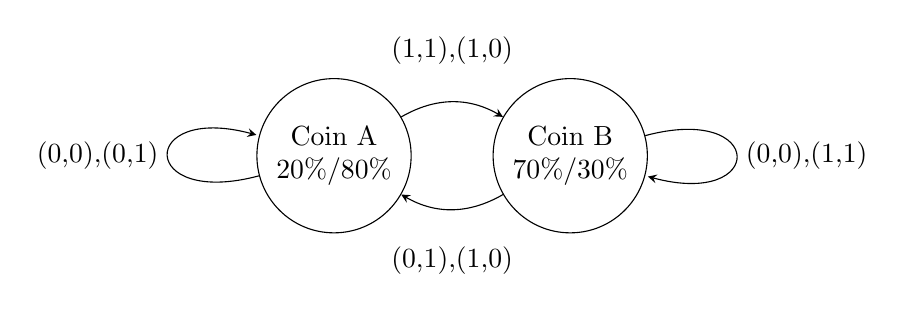
\begin{tikzpicture}[->, >=stealth, node distance=3cm, auto, scale=1, transform shape]

    % Define states
    \node[state, align=center] (A) {Coin A\\20\%/80\%};
    \node[state, right of=A, align=center] (B) {Coin B\\70\%/30\%};

    % Transitions
    \path   (A) edge [loop left]  node              {(0,0),(0,1)} (A)
                edge [bend left]  node[yshift=1em]  {(1,1),(1,0)} (B)
            (B) edge [loop right] node              {(0,0),(1,1)} (B)
                edge [bend left]  node[yshift=-1em] {(0,1),(1,0)} (A);

\end{tikzpicture}
\label{fig:coin-system-example}
\caption{An example of a size $n=2$, memory depth $m=2$ coin system. Coin A has probability distribution $P_{A}=(20\%, 80\%)$ and Coin B has probability distribution $P_{B} = (70\%,30\%)$ for Heads (0) and Tails (1) respectively. The transition rules $T$ are defined based on every possible combination of all $n$ outputs of length $m$ and unique for each coin in the system. For example, $T_{A}(0,0) \rightarrow A$ but $T_{B}(0,0) \rightarrow B$.}
\end{figure}

For example, a coin system containing two coins with two outputs ($n=2$) with a memory depth of $m=2$ is shown in figure \ref{fig:coin-system-example}, and numerically, it could be represented through the use of a $2 \times 2$ square matrix representing the probabilities and a lookup table for the transition rules.

\begin{table}[H]
\centering
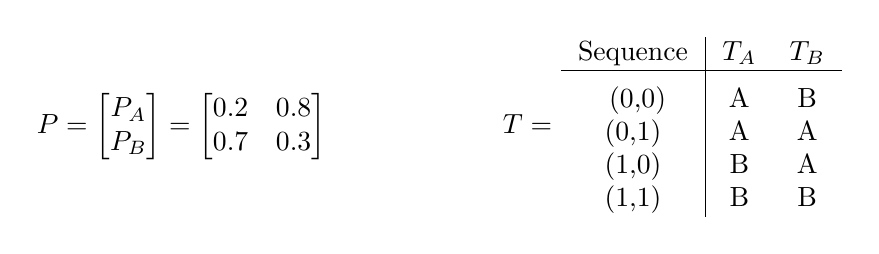
\begin{tikzpicture}

    % Transition Matrix (Left Side)
    \node (T) {$P = \begin{bmatrix} P_A \\ P_B \end{bmatrix} = 
    \begin{bmatrix} 0.2 & 0.8 \\ 0.7 & 0.3 \end{bmatrix}$};

    % Table (Right Side)
    \node (M) [right=2cm of T] {
        $T =$
        \begin{tabular}{c|c c}
            Sequence & $T_{A}$ & $T_{B}$ \\ 
            \hline\rule{0pt}{13pt}
            (0,0) & A & B \\
            (0,1) & A & A \\
            (1,0) & B & A \\
            (1,1) & B & B \\
        \end{tabular}
    };

\end{tikzpicture}
\label{tbl:coin-system-numerical-description}
\caption{A continuation of the example shown in figure \ref{fig:coin-system-example}, displaying the probabilities $P$ as a square matrix of size $n \times n$ and the transition rules as a lookup table mapping a series of outputs $m$ long to the next coin in the chain based on the present coin.}
\end{table}

Commonly, the transition rules between states for a Markov chain is also defined using an $n \times n$ matrix in the form of a transition probability distribution, but in this case, we've opted to have explicit rules for each transition rather than a probability due to our outputs and states being distinct (the outputs and states are not the same thing for a coin system, but they are for problems like weather modeling), and because it allows us to explicitly define a memory-depth. Additionally, in the case that a transition matrix may be necessary (such as analytically calculating the standing distribution), this still could be calculated using the probability distribution and the transition rules, but it was not necessary for this project.

Additionally, in this study, two key statistics are used for analyzing the behavior of these models: complexity and error. Every model has a complexity rating (denoted $c$) defined by the formula
\begin{equation}\label{eq:complexity}
c = nvm^2,
\end{equation}
where $n$ is the size of the model, $m$ is the memory depth, and $v$ is the system-wide variance of the model. 

System-wide variance is defined as the sum of the individual variance for every output on every coin of the model by equation
\begin{equation}\label{eq:sw-variance}
    v = \sum_{i=1}^{n} Var(S_{i}),
\end{equation}
where $S_{i}$ is coin (or state) $i$ in the system.

Individual variance is defined as the absolute difference of an output from its expected, unbiased equivalent ($100\%$ divided by the number of outputs), thus coin-wide variance is defined as
\begin{equation}\label{eq:ind-variance}
    Var(S) = \sum_{i=1}^{n} |P_{S,i} - \mu|,
\end{equation}
where $P_{S,i}$ is the probability for output $i$ on coin $S$, and $\mu = \frac{1}{n}$ is the unbiased probability.

By the law of large numbers, each of these models is guaranteed to converge to a certain long-term probability distribution when run to produce an infinitely long series of outputs. This distribution can calculated analytically using the probability matrix $P$ and a transition matrix (which, as mentioned before, we could calculate) or determined experimentally, and for the sake of ease, we chose to simply determine it experimentally for each model (which we refer to as the experimental probability distribution or EPD). Any mismatch in the standing distributions of two models guarantees that there is error (or dissimilarity) between the two models, but a match does not guarantee similarity as multiple models with considerably different internal weights can have the same standing distribution.

As such, we chose to define error as the product of the absolute difference sums between their probabilities and EPDs,
\begin{equation}
    E(I,O) = |EPD_{I} - EPD_{O}| \times |P_{I} - P_{O}|,
\end{equation}
where $I$ is the input model (the "true" model, before reverse-engineering) and $O$ is the output model (the reverse-engineered model).

\subsection{Testing}

For each test, we randomly generated 1000 coin systems, each with psuedo-random weights (probabilities and transition rules) within a range of $n \in \{1, 2, 3, 4, 5\}$ and $m \in \{1, 2, 3, 4\}$, with each initially-generated model referred to as the "input model." The input model was then run/flipped to produce a sequential list of outputs $L=10^4$ long, and from this list, the empirical standing distribution of the model is calculated. Then, this sequence of outputs and select data about the model is passed into each of the solvers (see table \ref{tbl:algorithms})
\end{document}